\documentclass[10pt,twocolumn,letterpaper]{article}

\usepackage{cvpr}
\usepackage{times}
\usepackage{epsfig}
\usepackage{graphicx}
\usepackage{amsmath}
\usepackage{amssymb}
\usepackage{pifont}
\usepackage{subcaption}

\usepackage[breaklinks=true,bookmarks=false]{hyperref}

\cvprfinalcopy

\def\httilde{\mbox{\tt\raisebox{-.5ex}{\symbol{126}}}}

\begin{document}

\title{Neural Image Style Transfer: Color Preservation and Video Support}

\author{Christina Sun\\
6.869\\
{\tt\small sunc@mit.edu}
\and
Larry Zhang\\
6.869\\
{\tt\small larryq@mit.edu}
}

\maketitle

\begin{abstract}
  We extend the neural artistic style transfer algorithm, which generates an output image that has the same content of one image and the same style of another. While the original algorithm allows for automatic creation of new artwork in the style of famous painters and artistic movements, it is unable to retain color information from the content image. In this report, we implement and explore three extensions to the neural style transfer algorithm that preserve content color. We also implement a simple method that extends the algorithm to support style transfer in video content.
\end{abstract}

\section{Introduction}
Neural style transfer has automated the otherwise painstaking manual process of creating artwork that is reminiscent of a particular style or artist. One of the more effective algorithms for image style transfer was originally proposed in~\cite{gatys-orig}, which uses feature matching in a pre-trained convolutional neural network (CNN) to generate a new image containing the content of one image with the style of another. For example, Figure~\ref{fig:orig} shows a path with flowers as the content image and Robert Delaunay's \textit{Portrait de Jean Metzinger} as the style image. The algorithm uses these two images to then generate an image containing the same path with flowers, but stylized with Delaunay's painting.

\begin{figure*}[ht]
\centering
\begin{subfigure}[b]{0.38\linewidth}
  \centering
  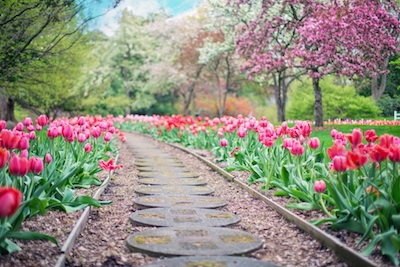
\includegraphics[width=\linewidth]{imgs/flowers.jpg}
  \caption{Content}
\end{subfigure}
\quad
\begin{subfigure}[b]{0.19\linewidth}
  \centering
  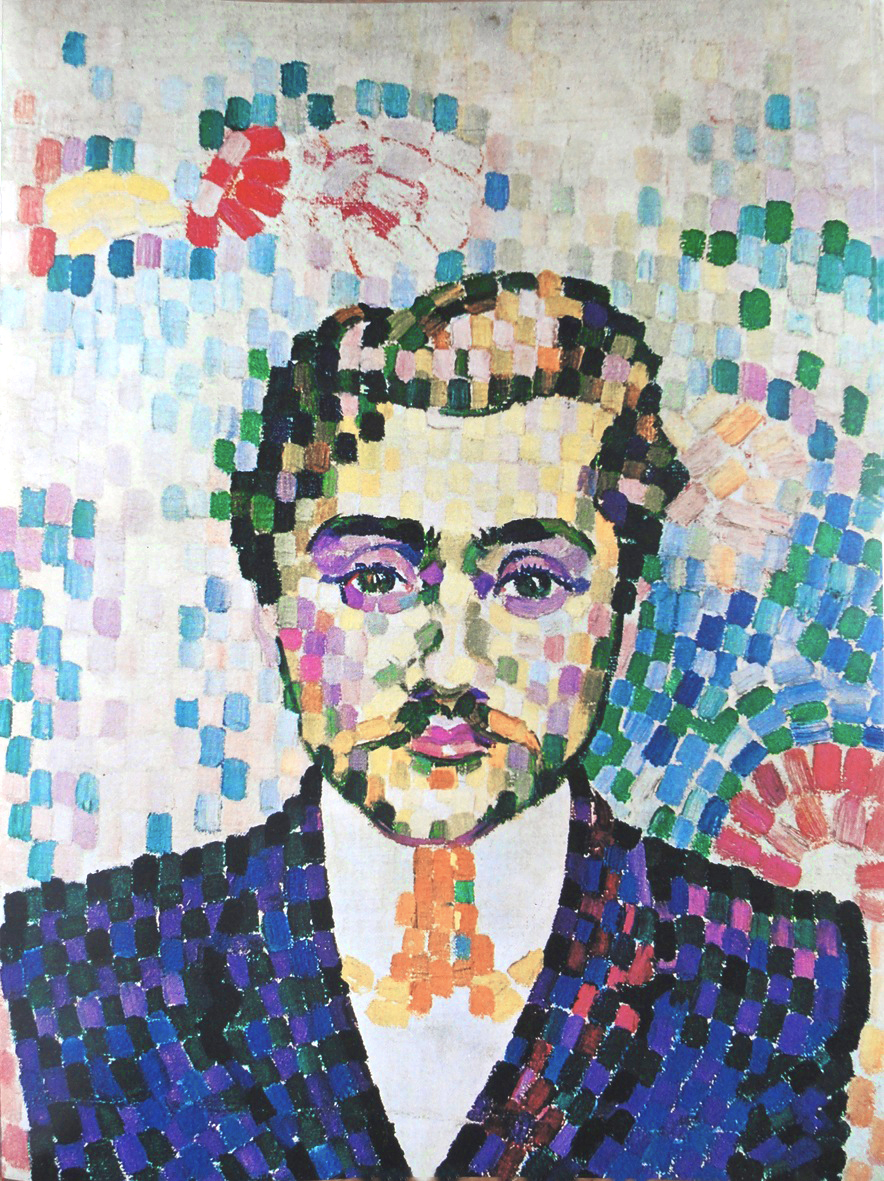
\includegraphics[width=\linewidth]{imgs/delaunay.jpg}
  \caption{Style}
\end{subfigure}
\quad
\begin{subfigure}[b]{0.38\linewidth}
  \centering
  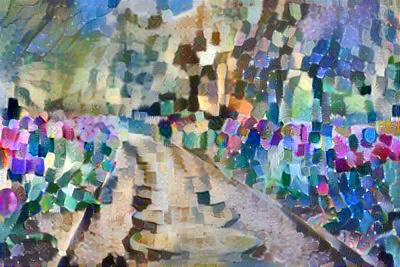
\includegraphics[width=\linewidth]{imgs/flowers-delaunay.jpg}
  \caption{Output}
\end{subfigure}
\caption{Example of neural image style transfer. (a)~Input image. (b)~Robert Delaunay's \textit{Portrait de Jean Metzinger}. (c)~Output image generated using the algorithm from~\cite{gatys-orig}.}
\label{fig:orig}
\end{figure*}

From Figure~\ref{fig:orig}, we see that while the output successfully transfers the brushstrokes and overall geometry of the style image, it also transfers the style's color distribution, thus losing the original colors of the content image. In this report, we explore a few methods for preserving the colors of the input image.

Additionally, the original method described in ~\cite{gatys-orig} applies strictly to transferring the style of an image to another image. We also explore an extension to the original algorithm that attempts to transfer the style of an image to an entire video sequence.

\section{Related Work}
At a high level, neural style transfer involves modifying an initial image consisting of white noise and iteratively changing pixels to resemble a desired target whose content is similar to the content image, and whose style is similar to the style image. To achieve this effect, the algorithm back-propagates the outputs of various layers of a pretrained CNN model in order to minimize the content and style losses. As a result, the initial random noise transforms into an image with the desired content and style.

\subsection{Color Preservation}
In~\cite{gatys-color}, the same author of the original neural style transfer algorithm explores two methods for preserving color in the output image.

The first, which we refer to as color mapping, attempts to transform the original style image $S$ so that its colors match those of the content image $C$. This new style image $S'$ with corrected colors is then used in the original neural style transfer algorithm.

The actual color mapping algorithm employs a simple linear transform that shifts the mean and covariance of the RGB values of the style image to match those of the content image:
\begin{equation}\label{eq:cov}
  x_{S'} = \Sigma_C^\frac{1}{2}\Sigma_S^{-\frac{1}{2}} (x_S - \mu_S) + \mu_C,
\end{equation}
where $x_i = [R, G, B]^T$ represents a pixel in image $i$, $\mu_S$ and $\mu_C$ are the mean colors of the style and content images, and $\Sigma_S$ and $\Sigma_C$ are the pixel covariances.

The second method described in~\cite{gatys-color} is called luminance transfer. After the neural style transfer algorithm generates an output image $O$, both $O$ and $C$ are converted into the YIQ colorspace. Because the original color information of the content image is represented by its $I$ and $Q$ channels, the correctly colored output is simply the combination of $Y_O$, $I_C$, and $Q_C$.

\begin{figure*}[ht]
\centering
\begin{subfigure}[b]{0.48\linewidth}
  \centering
  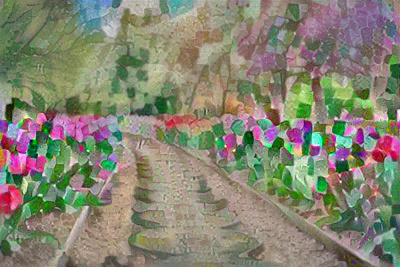
\includegraphics[width=\linewidth]{imgs/flowers-rgb-eig.jpg}
  \caption{Color mapping}
\end{subfigure}
\quad
\begin{subfigure}[b]{0.48\linewidth}
  \centering
  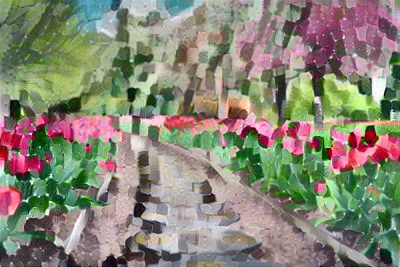
\includegraphics[width=\linewidth]{imgs/flowers-luminance.jpg}
  \caption{Luminance transfer}
\end{subfigure}
\caption{Comparison of the two color preservation methods from~\cite{gatys-color}.}
\label{fig:color-orig}
\end{figure*}

Figure~\ref{fig:color-orig} shows a comparison of the color mapping and luminance transfer methods from~\cite{gatys-color}. As explained in the paper, luminance transfer better preserves the color of the content image, but loses the relationship between the luminance and color channels. Specifically, in styles with prominent brushstrokes, as in Delaunay's art, the output will likely have strokes that do not align with the colors. We believe that this dependency is an important aspect of style transfer, and thus explore improvements to the color mapping algorithm that better preserve content color.

\subsection{Video}
The simplest and most common approach for applying neural style to a video is to extract the sequence of frames and individually pass each image into the algorithm, as in regular neural style transfer. More sophisticated approaches use more intelligent initialization images, rather than random noise. In~\cite{video1}, the authors enforce a constraint that encourages minimal deviations between two frames that accounts for extreme movement and occlusions. The authors of~\cite{video2} also explore other loss functions that maintain temporal consistency between frames, while still maintaining reasonable processing time.

\section{Approach}
We utilize an open-source tensorflow implementation of the original neural style transfer algorithm~\cite{neuralstyle}. This implementation uses a VGG19 CNN pretrained on the ImageNet dataset~\cite{vgg}. All color and video extensions are integrated with the open-source implementation for end-to-end functionality. All images in this report were generated after 1000 iterations of the algorithm.

\subsection{Color Preservation}
To improve the color mapping algorithm presented in~\cite{gatys-color}, we look at modifying the transformation used to match the colors of the style image with those of the content image. Rather than simply performing a linear shift and rescaling on the RGB values of the style image, we explore three color mapping algorithms described in~\cite{color}. Each of these algorithms produces a color-mapped version of the style image, which is then used with the content image in neural style transfer.

\bigbreak\noindent\textbf{Different colorspaces.}
Working with individual channels of the RGB colorspace may not be ideal since the channels are highly correlated. By using a less correlated colorspace, we can linearly shift and scale each channel independently without worrying about inter-channel relationships. Here, we explore two colorspaces, $l\alpha\beta$~\cite{lab} and YUV.

In the case of both colorspaces, we first convert the style image $S$ and content image $C$ into the colorspace. Then, for each $l\alpha\beta$ or YUV channel in $S$, we independently shift the mean and scale the standard deviation of the pixel values in that channel so that they match those in $C$:
\begin{equation}\label{eq:std}
  x_{S'} = \frac{\sigma_C}{\sigma_S} (x_S - \mu_S) + \mu_C,
\end{equation}
where $x_i = [l, \alpha, \beta]^T$ or $[Y, U, V]^T$ represents a pixel in image $i$, and $\mu_i$ and $\sigma_i$ are the mean and standard deviation of pixel values in that image. Finally, we shift the generated image $S'$ back to RGB. Note that Equation~(\ref{eq:std}) is very similar to Equation~(\ref{eq:cov}) used in~\cite{gatys-color}. While both are linear transformations, the important distinction is that, since we are treating each channel independently, we are calculating standard deviations and not a covariance matrix.

\bigbreak\noindent\textbf{PCA transform.}
Even though the $l\alpha\beta$ and YUV colorspaces are less correlated than RGB, they both have their respective limitations and are not perfectly uncorrelated. Thus, rather than working with predefined colorspaces, we can compute an uncorrelated colorspace for each of the images using principal component analysis (PCA). Thus, rather than transforming pixel values according to the $l\alpha\beta$ or YUV colorspaces, we use the principal components of each image~\cite{pca}.

More formally, let $PC_S$ and $PC_C$ be the principal components of the style and content images, respectively. Using $PC_S$, we transform the pixels of the style image from RGB into the principal component space. We then use $PC_C$ to inversely transform these pixels from the principal component space back into RGB to generate $S'$. This transform will ensure that the principal components of $S'$ are equal to those of the content image.

\bigbreak\noindent\textbf{Random rotations.}
Another approach for color mapping utilizes randomization to iteratively reshape one distribution to match another target distribution~\cite{random}. In our case, the pixels in the style image represent the starting 3D color distribution, and the pixels in the content image represent the target distribution. At each step of the iteration, the style pixels $S$ and content pixels $C$ are rotated using a random 3D rotation matrix $R$~\cite{randrot} to produce $S_R$ and $C_R$. Then, independently with respect to each of the three axes in this rotated space, the distribution $S_R$ is shifted and scaled to match that of $C_R$. We use the same linear transformation from Equation~(\ref{eq:std}) for simplicity (mean and standard deviation matching). The resulting distribution $S'_R$ is then rotated back to the original (RGB) space to produce $S'$. This process is then repeated using $S'$ (instead of $S$) with a different rotation matrix until convergence.

The updates during a single iteration are summarized below:
\begin{align}
  S_R &= R S \\
  S_C &= R C \\
  x_{S'_R} &= \frac{\sigma_{C_R}}{\sigma_{S_R}} (x_{S_R} - \mu_{S_R}) + \mu_{C_R} \\
  S' &= R^{-1} S'_R \\
  S &\leftarrow S'
\end{align}
where $x_i$ represents a pixel in image $i$ in the rotated space defined by $R$.

\subsection{Video}
To extend the neural style transfer algorithm to work with video content, we directly feed individual frames into the algorithm. The original, unmodified implementation initializes each frame with random noise. Therefore, the styles of the outputs may emerge differently for consecutive frames. The stylized video will appear segmented and jittery, since there is no continuity between frames. This is emphasized by the circles in Figure~\ref{fig:video-orig}, which highlight a dramatic style difference between two consecutive output frames in a video sequence. The entire video using the original neural style implementation can be viewed at \url{https://media.giphy.com/media/l3mZ1zQv2uObq9kKk/giphy.gif}.

\begin{figure*}[ht]
\centering
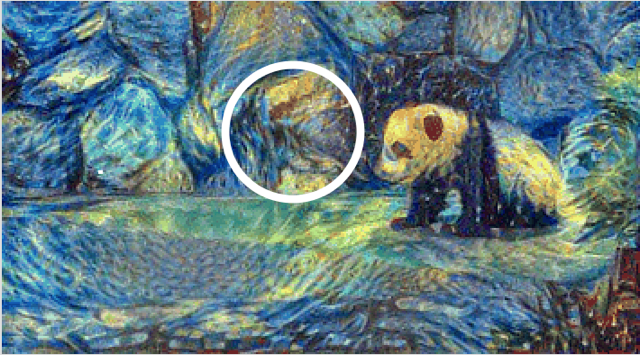
\includegraphics[width=0.48\linewidth]{imgs/panda1.png}
\quad
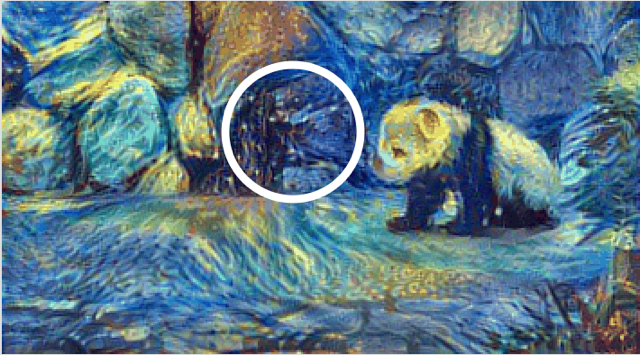
\includegraphics[width=0.48\linewidth]{imgs/panda2.png}
\caption{Two consecutive frames of a stylized video sequence. The circles emphasize stylistic discontinuity between the two consecutive frames, which causes the resulting video to jitter.}
\label{fig:video-orig}
\end{figure*}

Our approach to mitigating this problem is to initialize each frame with the output of the previous frame. This way, instead of generating a new output from random noise, we are using a visually similar image as a starting point. Ideally, the calculated loss of this new initial image is smaller than that of random noise, so fewer updates are needed. In theory, this method also reduces computation time. Since the content and style do not change greatly between frames, we need fewer iterations to process frames after the first.

\section{Results}
\subsection{Color Preservation}
The results for each of the three color mapping algorithms are discussed below.

\bigbreak\noindent\textbf{Different colorspaces.}
Figure~\ref{fig:color-result} shows the results of performing neural style transfer using the style image generated by linearly matching the mean and standard deviation between the original content and style images. Channel statistics matching is performed independently in both the $l\alpha\beta$ and YUV colorspaces. For easy comparison, we use the same content image as before (path with flowers).

\begin{figure*}[ht]
\centering
\begin{subfigure}[b]{0.48\linewidth}
  \centering
  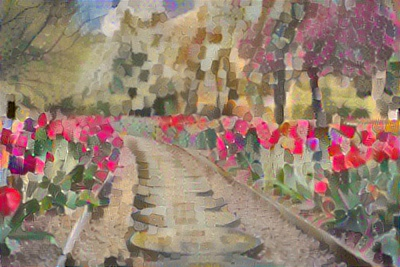
\includegraphics[width=\linewidth]{imgs/flowers-lab-lin.jpg}
  \caption{$l\alpha\beta$ colorspace}
\end{subfigure}
\quad
\begin{subfigure}[b]{0.48\linewidth}
  \centering
  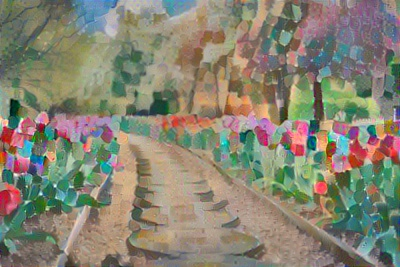
\includegraphics[width=\linewidth]{imgs/flowers-ycbcr-lin.jpg}
  \caption{YUV colorspace}
\end{subfigure}
\caption{Style transfer results after mean and standard deviation matching in the $l\alpha\beta$ and YUV colorspaces.}
\label{fig:color-result}
\end{figure*}

While both images still retain the dependence between luminance and color (colors remain constant withing individual strokes), neither preserves the original color distribution of the content image well. The $l\alpha\beta$ colorspace result seems to have a reddish hue, which is likely due to imperfect colorspace conversions (RGB must first be converted to XYZ before being converted into $l\alpha\beta$). The YUV colorspace result also contains artifacts of colors present in the original style image, but not in the original content image (teal-colored flowers and leaves).

\begin{figure*}[ht]
\centering
\begin{minipage}{0.48\linewidth}
\centering
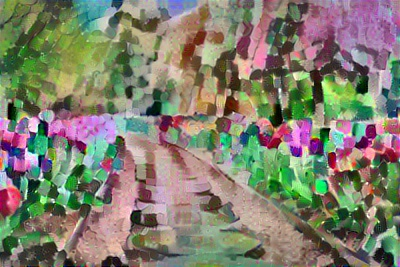
\includegraphics[width=\linewidth]{imgs/flowers-rgb-pca.jpg}
\caption{Style transfer result after principal component matching.}
\label{fig:pca-result}
\end{minipage}
\quad
\begin{minipage}{0.48\linewidth}
\centering
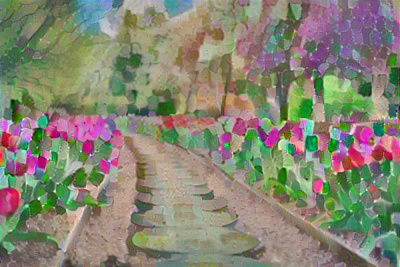
\includegraphics[width=\linewidth]{imgs/flowers-rgb-rot.jpg}
\caption{Style transfer result after random rotation matching.}
\label{fig:rot-result}
\end{minipage}
\end{figure*}

\bigbreak\noindent\textbf{PCA transform.}
Figure~\ref{fig:pca-result} shows the result of performing neural style transfer using the style image generated by matching the principal components of the original content and style images. We again use the same content image as before.

The colors in this image are much more similar to those in the original content image. However, the image's contrast is unnatural and unrepresentative of the content's color distribution. This is because our PCA method will effectively rotate the pixel values to match in color, but does nothing to regulate the variance in the rotated values. Thus, the high variance in the intensity of pixels in the Delaunay style image is also transferred to the result, causing higher contrast in the output.

\bigbreak\noindent\textbf{Random rotations.}
Figure~\ref{fig:rot-result} shows the result of performing neural style transfer using the style image generated by using the random rotations method. We use the same content image as before.

Visually, this approach seems to produce the best results in terms of matching the original colors from the content image. Thus, it leverages the benefits from both the original color mapping and luminance transfer algorithms described in~\cite{gatys-color}: color is accurately preserved in the output image, and dependency between luminance and color is maintained.

\subsection{Video}
\begin{figure*}[ht]
\centering
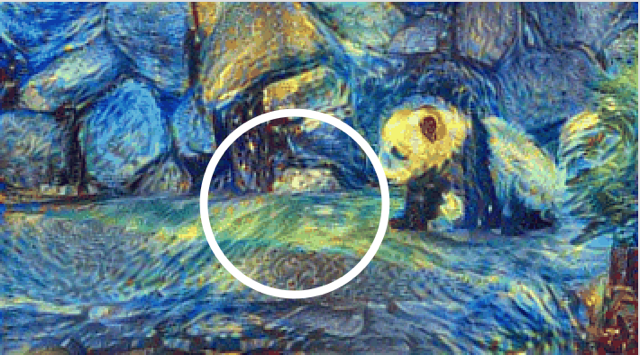
\includegraphics[width=0.48\linewidth]{imgs/pandap1.png}
\quad
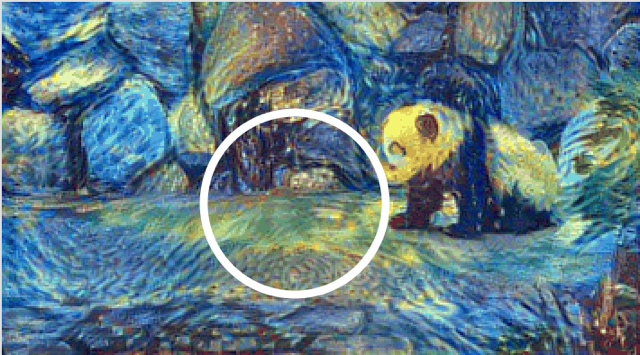
\includegraphics[width=0.48\linewidth]{imgs/pandap2.png}
\caption{Two consecutive frames of a stylized video sequence where the previous output is used in initialization. Circled regions are now more visually similar to each other.}
\label{fig:video-final}
\end{figure*}

The results of using the output of each frame as the initialization image of the next frame can be found at \url{https://media.giphy.com/media/3oxHQgEvUcU8kvOifS/giphy.gif}. Figure~\ref{fig:video-final} shows two consecutive frames of the new video output. Observe that the circled parts of the frames are more similar in terms of stroke color, shape, and orientation than the example in Figure~\ref{fig:video-orig}.

When viewing the entire video sequence, however, there is still a significant amount of discontinuity between frames. This occurs because the loss calculation in neural style transfer is computed per pixel, and thus does not take into account regional similarities. When pixel values shift between frames due to movement in the scene, the initial image may visually look like our desired target, but the pixel-based loss may still be large. Thus, the calculated updates from back-propagation may still result in dramatic differences between consecutive frames. To improve upon this method, we would explore ways to penalize large discrepancies between consecutive video frames, such as enforcing consistency through the use of a different loss function.

Because our generated videos did not maintain temporal consistency, we did not explore reducing the required processing time for frames after the first.

\section{Conclusion}
Many recent advances in neural style transfer have automated the process of creating artwork with a specific style. While these methods accurately capture the style and content of the input images, other details such as color, are not so effectively transferred. However, this preservation may be desired. We explore three different methods for preserving color: color mapping using different colorspaces, PCA transformation, and random rotations. We also implement neural style transfer from images to videos. We show that initializing the image with the output of the previous frame results in a slightly less jarring viewing experience.

\subsection{Future Work}
Our PCA color mapping implementation transfers intensity variation from the style image to the newly generated one. Thus, future work will involve regulating this variance by taking into account the variance explained by each of the principal components.

The random rotation color mapping, though effective, can also be improved. We use simple linear mean and standard deviation matching in the rotated space, but more complex matching may generate better results. For example, histogram matching in the rotated space will generate a style image with a color distribution much closer to that of the content image.

Finally, for video support, we would like to explore the use of a more sophisticated loss function that will effectively encourage continuity between consecutive frames. We would also investigate if this new method can be used to decrease computation time by reducing the number of iterations required to generate frames past the first.

\section{Individual Contribution}
Together with Christina, we read through the relevant previous work to ensure that both of us had a good understanding of how neural style transfer worked. Later, we collaboratively set up the open-source neural style transfer model. I then focused on improving the model to preserve color in the output, while Christina focused on adding style transfer functionality for video. We met frequently to help each other with pain points, and ultimately wrote the paper together.

{\small
\bibliographystyle{ieee}
\bibliography{bib}
}

\end{document}
